% PDF Looker Pro: an open-source annotating PDF reader.
%
% Build: pdflatex main.tex && pdflatex main.tex  (two passes for references)
% arXiv: upload this file together with sections/ and figures/ (see paper/README.md).
\documentclass[11pt,a4paper]{article}

\usepackage[T1]{fontenc}
\usepackage[utf8]{inputenc}
\usepackage[margin=1in]{geometry}
\usepackage{newtxtext,newtxmath}
\usepackage{microtype}
\usepackage{booktabs}
\usepackage{graphicx}
\usepackage{xcolor}
\usepackage{tikz}
\usetikzlibrary{arrows.meta,positioning,fit,backgrounds,shapes.misc}
\usepackage{listings}
\usepackage{caption}
\usepackage{enumitem}
\usepackage{amsmath}
\usepackage[hidelinks]{hyperref}
\usepackage{url}

\hypersetup{
  pdftitle={PDF Looker Pro: an open-source annotating PDF reader and document editor},
  pdfsubject={Software engineering; document formats},
  pdfauthor={Chengxi Zhang},
}

\definecolor{ink}{HTML}{1F2937}
\definecolor{grey}{HTML}{6B7280}
\definecolor{accent}{HTML}{1F6FEB}
\definecolor{codebg}{HTML}{F6F8FA}

\lstdefinestyle{pdf}{%
  basicstyle=\ttfamily\footnotesize\color{ink},
  backgroundcolor=\color{codebg},
  frame=single, framerule=0.3pt, rulecolor=\color{grey!40},
  breaklines=true, breakatwhitespace=false,
  columns=fullflexible, keepspaces=true,
  showstringspaces=false, xleftmargin=4pt, xrightmargin=4pt,
  aboveskip=6pt, belowskip=6pt,
}
\lstset{style=pdf}

\setlist[itemize]{leftmargin=1.4em,itemsep=1pt,topsep=3pt}
\setlist[enumerate]{leftmargin=1.6em,itemsep=1pt,topsep=3pt}

\captionsetup{font=small,labelfont=bf}
\renewcommand{\arraystretch}{1.12}

% Numbers reported in this paper were measured on the artefact; the scripts that
% produce them live in the repository (tools/collect-metrics.mjs, tools/benchmark.mjs)
% and their raw output is in paper/metrics/.
\newcommand{\repo}{\url{https://github.com/dongfangxy/pdf-looker-pro}}

\title{\bfseries PDF Looker Pro: an open-source annotating PDF reader\\ and document editor}

\author{%
  Chengxi Zhang\\
  \small Independent researcher\\
  \small\href{mailto:dongfangxy@163.com}{\texttt{dongfangxy@163.com}}
}
\date{October 2026}

\begin{document}
\maketitle

\begin{abstract}
\noindent
Portable Document Format (PDF) readers are abundant, but open-source readers that
\emph{write} into a PDF rather than beside it are not: most either render the page and keep
annotations in a sidecar, or depend on a large commercial-grade engine. This paper
describes \textbf{PDF Looker Pro}, a desktop PDF reader, annotator and page editor whose
PDF layer is written from scratch in TypeScript and whose only runtime dependency is the
pdf.js rendering engine. We report the engineering rather than a new algorithm, because the
interesting failures in this kind of system are invariants that are easy to state and easy
to violate. Three are examined in detail: an incremental annotation writer must rebuild a
page's \texttt{/Annots} from ``existing minus replaced, plus new'' or it will duplicate
every annotation on every save and resurrect every deleted one; a whole-document rewrite
must materialise attributes a page previously inherited, or flattening the page tree
silently resizes and reorients it; and merging two documents must renumber every reference
in the incoming object graph while copying stream bytes verbatim. The annotation model
keeps two representations of each mark, a standard subtype for interoperability and a
private dictionary for lossless round-tripping, and the paper is explicit about the cost of
that duality. The system is verified by 789 behavioural assertions over 31 suites --- 734 against the
browser build and 55 against the packaged application --- and we report the defects that
methodology caught, including one the authors introduced into the harness itself, together
with the case in which it gave a false sense of coverage. The application is 17{,}323 lines of source over 47 files,
MIT licensed, and publicly available.
\end{abstract}

\vspace{0.4em}
\noindent\textbf{Keywords:} PDF, document formats, annotation, incremental update,
software verification, Electron

\section{Introduction}
\label{sec:intro}

A PDF file is a program for a printer: a page tree, content streams, fonts, and a
cross-reference index that says where every object lives. Readers are therefore easy to
classify by what they do with those bytes. A \emph{renderer} reads them. A \emph{reader with
comments} either writes new objects into the file --- which changes the bytes other
applications see --- or keeps annotations in a companion file, which the reader next to it
will never show.

The distinction matters because a PDF is usually not the only copy. An annotated manuscript
is mailed to a co-author, a marked-up drawing goes to a fabricator, a reviewed contract goes
back to a lawyer. An annotation that lives in a sidecar reaches none of them.

Writing into a PDF is not hard to begin and hard to get right. The format is designed for
\emph{incremental} updates: append objects, rewrite the dictionaries that changed, add
another cross-reference section pointing back at the previous one, and the file remains valid
for every existing reader. The difficulty is that an update is a \emph{diff}, so every save
has to know what the previous save did. A writer that only appends is correct exactly once.

This paper reports what it took to build such a reader as a self-contained system:
\textbf{PDF Looker Pro}, an MIT-licensed desktop application for Windows whose PDF layer
--- parser, incremental writer, whole-document rewrite and merger --- is written from
scratch in TypeScript. The only runtime dependency is pdf.js~\cite{pdfjs}, used for
rasterisation and text extraction; the page model, the writers and the annotation model are
the authors' own. The feature set follows that of a long-standing commercial Windows viewer
for which development has ceased~\cite{pdfxchange}; there is no affiliation with it and no
code in common.

\paragraph{Contributions.} We claim no new algorithm. The contributions are an account of
the invariants that a system of this kind must satisfy, the design that satisfies them, and a
verification methodology with an honest record of what it caught and what it missed.

\begin{enumerate}
  \item \textbf{A deletion-correct incremental annotation writer}
        (\S\ref{sec:incremental}). A page's \texttt{/Annots} is rebuilt as
        \emph{(existing $\setminus$ replaced) $\cup$ new}, where ``replaced'' is the set of
        object numbers the previous save produced. A page whose annotations were all deleted
        is still rewritten, because nothing else removes an obsolete entry. We show the two
        user-visible symptoms of violating this invariant --- annotations duplicating on every
        save, and deleted annotations reappearing --- both of which occurred in this codebase
        and both of which are now covered by a regression test.

  \item \textbf{A whole-document rewrite that materialises inheritance}
        (\S\ref{sec:rewrite}). Flattening the page tree to support delete, insert, reorder,
        extract and crop destroys attributes a page inherited from intermediate
        \texttt{/Pages} nodes (\texttt{MediaBox}, \texttt{CropBox}, \texttt{Resources},
        \texttt{Rotate}, \texttt{UserUnit}). The rewrite writes them onto every page, copies
        objects verbatim when they are stored uncompressed, re-serialises those inside object
        streams, and recomputes the cross-reference.

  \item \textbf{Cross-document merging by reference renumbering}
        (\S\ref{sec:merge}). The incoming object graph is renumbered above the host's highest
        object number; every reference is rewritten, every stream's bytes are copied
        unchanged, and the incoming pages are rebuilt on the host's page tree.

  \item \textbf{A dual-representation annotation model} (\S\ref{sec:annot-model}) that writes
        a standard subtype so other readers display the mark, and a private dictionary so this
        reader restores it without loss. We state the cost: two representations can disagree,
        and the standard one cannot express everything the private one can.

  \item \textbf{Search over a virtualised document} (\S\ref{sec:search}) that highlights by
        rewriting the text layer's spans, so a painted match is aligned with the painted
        glyphs by construction, guarded by a comparison against the strings the index was
        built from.

  \item \textbf{A dual-target verification methodology} (\S\ref{sec:verification}): 789
        behavioural assertions over 31 suites, 734 driving a browser build and 55 driving the
        packaged Electron application as a real executable, with a case study of a defect the
        second target caught and of three defects the authors introduced into the harness
        itself.
\end{enumerate}

\paragraph{Scope.} The paper describes a desktop application, not a library or a format
extension. It does not claim conformance to any profile of ISO 32000~\cite{iso32000}, does not
handle encrypted documents for writing, and does not implement forms, digital signatures or
optical character recognition. Section~\ref{sec:limits} lists the limitations in full; we
regard that list as a deliverable, not a disclaimer.

\paragraph{Availability.} Source, tests, build scripts and the measurement scripts that
produced every number in this paper are at \repo, MIT licensed. The packaged Windows build is
published as a release artefact of the same repository.

\section{Background and related work}
\label{sec:related}

\paragraph{The format.} PDF is specified by ISO 32000-1~\cite{iso32000}. A file is a
sequence of indirect objects, a page tree under a catalogue, and a cross-reference table
that maps object numbers to byte offsets. Two properties matter here. First, the format
admits \emph{incremental updates}: a new section may be appended at the end of the file with
its own cross-reference table and a \texttt{/Prev} pointer to the previous one, so the
original bytes never move. Second, page attributes are \emph{inheritable} along the page
tree: a page that omits \texttt{/MediaBox} takes the nearest ancestor's.

Streams are stored as a dictionary followed by raw bytes whose length the dictionary
declares. The bytes may be compressed by any of several filters, and objects may be packed
into a compressed container called an object stream. A writer that wants to copy a stream
without decoding it must therefore preserve the bytes exactly and copy the filter
description; a writer that has to rewrite a reference \emph{inside} an object stream cannot
do so without decoding and re-encoding the container.

\paragraph{Rendering engines.} pdf.js~\cite{pdfjs} is a JavaScript PDF renderer, Apache-2.0
licensed, and the rendering engine of Firefox. It exposes a page model and a canvas
rasteriser, plus a text-extraction API that yields positioned glyph runs. MuPDF~\cite{mupdf}
is a C engine, dual-licensed AGPL/commercial, with annotation support. PDFium is the engine
inside Chromium. These are renderers first; writing is either absent or a secondary concern.

\paragraph{Readers and annotators.} Okular~\cite{okular} (KDE, Poppler-backed) and Evince
(GNOME) are mature open-source readers with annotation support that write annotations into
the document through their respective back ends. Apache PDFBox~\cite{pdfbox} and iText are
libraries with full writing support, used by other applications rather than being
applications themselves. PDF-XChange Viewer~\cite{pdfxchange}, whose feature set this project
follows, is a commercial Windows viewer that is no longer developed.

The gap this project occupies is deliberately narrow: an \emph{application}, in which the
reader, the writers and the annotation model are open and readable together, with no engine
dependency beyond rasterisation, and with the writing logic documented as a set of invariants
rather than as behaviour to be discovered. We do not claim to be better at rendering, and we
do not compare rendering quality against the systems above; \S\ref{sec:eval} explains why
such a comparison would be neither fair nor useful at this stage.

\paragraph{Why write at all.} A sidecar annotation file is simpler in every engineering
respect: no incremental updates, no object numbering, no risk of corrupting the document. It
is also invisible to every other application. The design decision recorded here is that the
document is the artefact that travels, so the annotations must travel inside it. The price is
paid in \S\ref{sec:pdf-layer}.

\begin{table}[t]
  \centering
  \caption{Dependencies. The application's only runtime dependency is the rendering engine.
  Everything else is a build or verification tool and ships in no artefact.}
  \label{tab:deps}
  \small
  \begin{tabular}{@{}llll@{}}
    \toprule
    Package & Role & Version & Licence \\
    \midrule
    \texttt{pdfjs-dist} & rendering and text extraction & 5.x & Apache-2.0 \\
    \midrule
    \multicolumn{4}{@{}l}{\emph{build and verification only}} \\
    \texttt{electron} & desktop host & 44.x & MIT \\
    \texttt{electron-builder} & packaging & 26.x & MIT \\
    \texttt{vite} & bundler & 7.x & MIT \\
    \texttt{typescript} & type checker (erased at build) & 5.9 & Apache-2.0 \\
    \texttt{playwright} & browser and Electron driving & 1.64 & Apache-2.0 \\
    \bottomrule
  \end{tabular}
\end{table}

\section{System architecture}
\label{sec:arch}

The application is an Electron~\cite{electron} shell around a TypeScript renderer. The shell
owns windows, the native menu, file dialogues and printing; the renderer owns everything
else. The renderer is bundled by Vite~\cite{vite} into a single script of 660.2\,kB
(197.8\,kB gzip) plus 26.1\,kB of CSS (6.0\,kB gzip). User-interface resources ---
icons and strings that are not code --- are packed into a 19\,kB container with a format of
the project's own, described in the repository.

\begin{figure}[t]
\centering
% Explicit coordinates and a fixed text width: relative placement let a satellite box
% drift over its neighbour, and a figure that is wrong is worse than one that is plain.
\tikzset{
  box/.style={draw=ink!55, rounded corners=2pt, fill=white, align=center,
              font=\small, inner sep=3.2pt, text width=3.5cm, minimum height=8mm},
  side/.style={box, font=\footnotesize, text width=2.7cm, minimum height=7.4mm},
  group/.style={draw=grey!55, dashed, rounded corners=4pt, inner sep=6pt, fill=none},
  lbl/.style={font=\scriptsize\itshape, color=grey},
  ar/.style={-{Latex[length=1.6mm]}, draw=ink!65, thick},
  dep/.style={-{Latex[length=1.6mm]}, draw=ink!45, densely dashed},
}
\begin{tikzpicture}

% left column: the desktop shell
\node[box] (shell) at (0,0) {Electron main process\\\scriptsize windows, menu, dialogues, printing};
\node[box] (bridge) at (0,-1.35) {preload bridge\\\scriptsize typed, explicit surface};

% right column: the renderer
\node[box] (boot) at (7.0,0) {bootstrap\\\scriptsize \texttt{main.ts}, 91 commands};
\node[box] (viewer) at (7.0,-1.35) {viewer\\\scriptsize page list, virtualisation, zoom};
\node[box] (layer) at (7.0,-2.7) {annotation layer\\\scriptsize geometry, gestures, hit test};
\node[box] (model) at (7.0,-4.05) {annotation model\\\scriptsize kinds, store, history};
\node[box] (pdf) at (7.0,-5.4) {PDF layer\\\scriptsize parse $\cdot$ write $\cdot$ rewrite $\cdot$ merge};
\node[box] (engine) at (7.0,-6.75) {pdf.js\\\scriptsize rasterise, text runs};

% satellites, to the right of the column, well clear of it
\node[side] (tools) at (10.55,-2.7) {tools\\\scriptsize find, measure};
\node[side] (ui) at (10.55,-4.05) {UI\\\scriptsize dialogs, sidebar, i18n};

\begin{scope}[on background layer]
  \node[group, fit=(shell)(bridge), label={[lbl]above:desktop shell}] {};
  \node[group, fit=(boot)(viewer)(layer)(model)(pdf)(engine)(tools)(ui),
        label={[lbl]above:renderer (TypeScript, bundled)}] {};
\end{scope}

\draw[ar] (boot) -- (viewer);
\draw[dep] (layer) -- (model);
\draw[dep] (model) -- (pdf);
\draw[dep] (pdf) -- (engine);
\draw[dep] (tools.west) -- (layer.east);
\draw[dep] (ui.west) -- (model.east);
\draw[ar] (bridge.east) -- node[lbl, above]{\scriptsize IPC} (boot.west);
\end{tikzpicture}
\caption{Module layout. The PDF layer is the only component that touches bytes, and it is
independent of the renderer: it parses into its own value types rather than using pdf.js's
object model, which is what allows the writers to copy objects the renderer never looks at.
Solid arrows are calls; dashed arrows are use.}
\label{fig:arch}
\end{figure}

Figure~\ref{fig:arch} shows the layout and Table~\ref{tab:modules} its size. Two decisions
shape everything else.

\paragraph{The PDF layer has its own object model.} pdf.js exposes a document proxy that can
resolve objects, but it does not expose byte offsets, object generations, or the raw text of
an uncompressed object. All three are needed to write an incremental update: the offset is
what a cross-reference entry holds, the generation is part of a reference, and copying an
uncompressed object's bytes verbatim is both faster and safer than re-serialising a parse of
it. The project therefore has its own lexer and parser (\texttt{src/pdf}, eight files), and
uses pdf.js strictly as a rasteriser and text extractor. The duplication is real --- two
parsers over the same bytes --- and is the largest structural cost in the system; it buys
independence from a renderer's internal model, which is the property the writers need.

\paragraph{A page-space coordinate system of our own.} The renderer, the annotation model and
the hit test all work in \emph{unrotated page space at scale 1, origin top-left, $y$ down}.
PDF user space has its origin at the bottom-left and is scaled by the page's
\texttt{UserUnit}, so every conversion is explicit
($y_{\text{pdf}} = \texttt{MediaBox}_3 - y$) and every annotation stores coordinates that
survive a zoom, a rotation or a change of view mode without being rewritten. This sounds
pedantic and is not: the first implementation mixed rotated and unrotated coordinates and
placed marks correctly at 100\,\% and nowhere else.

\begin{figure}[t]
  \centering
  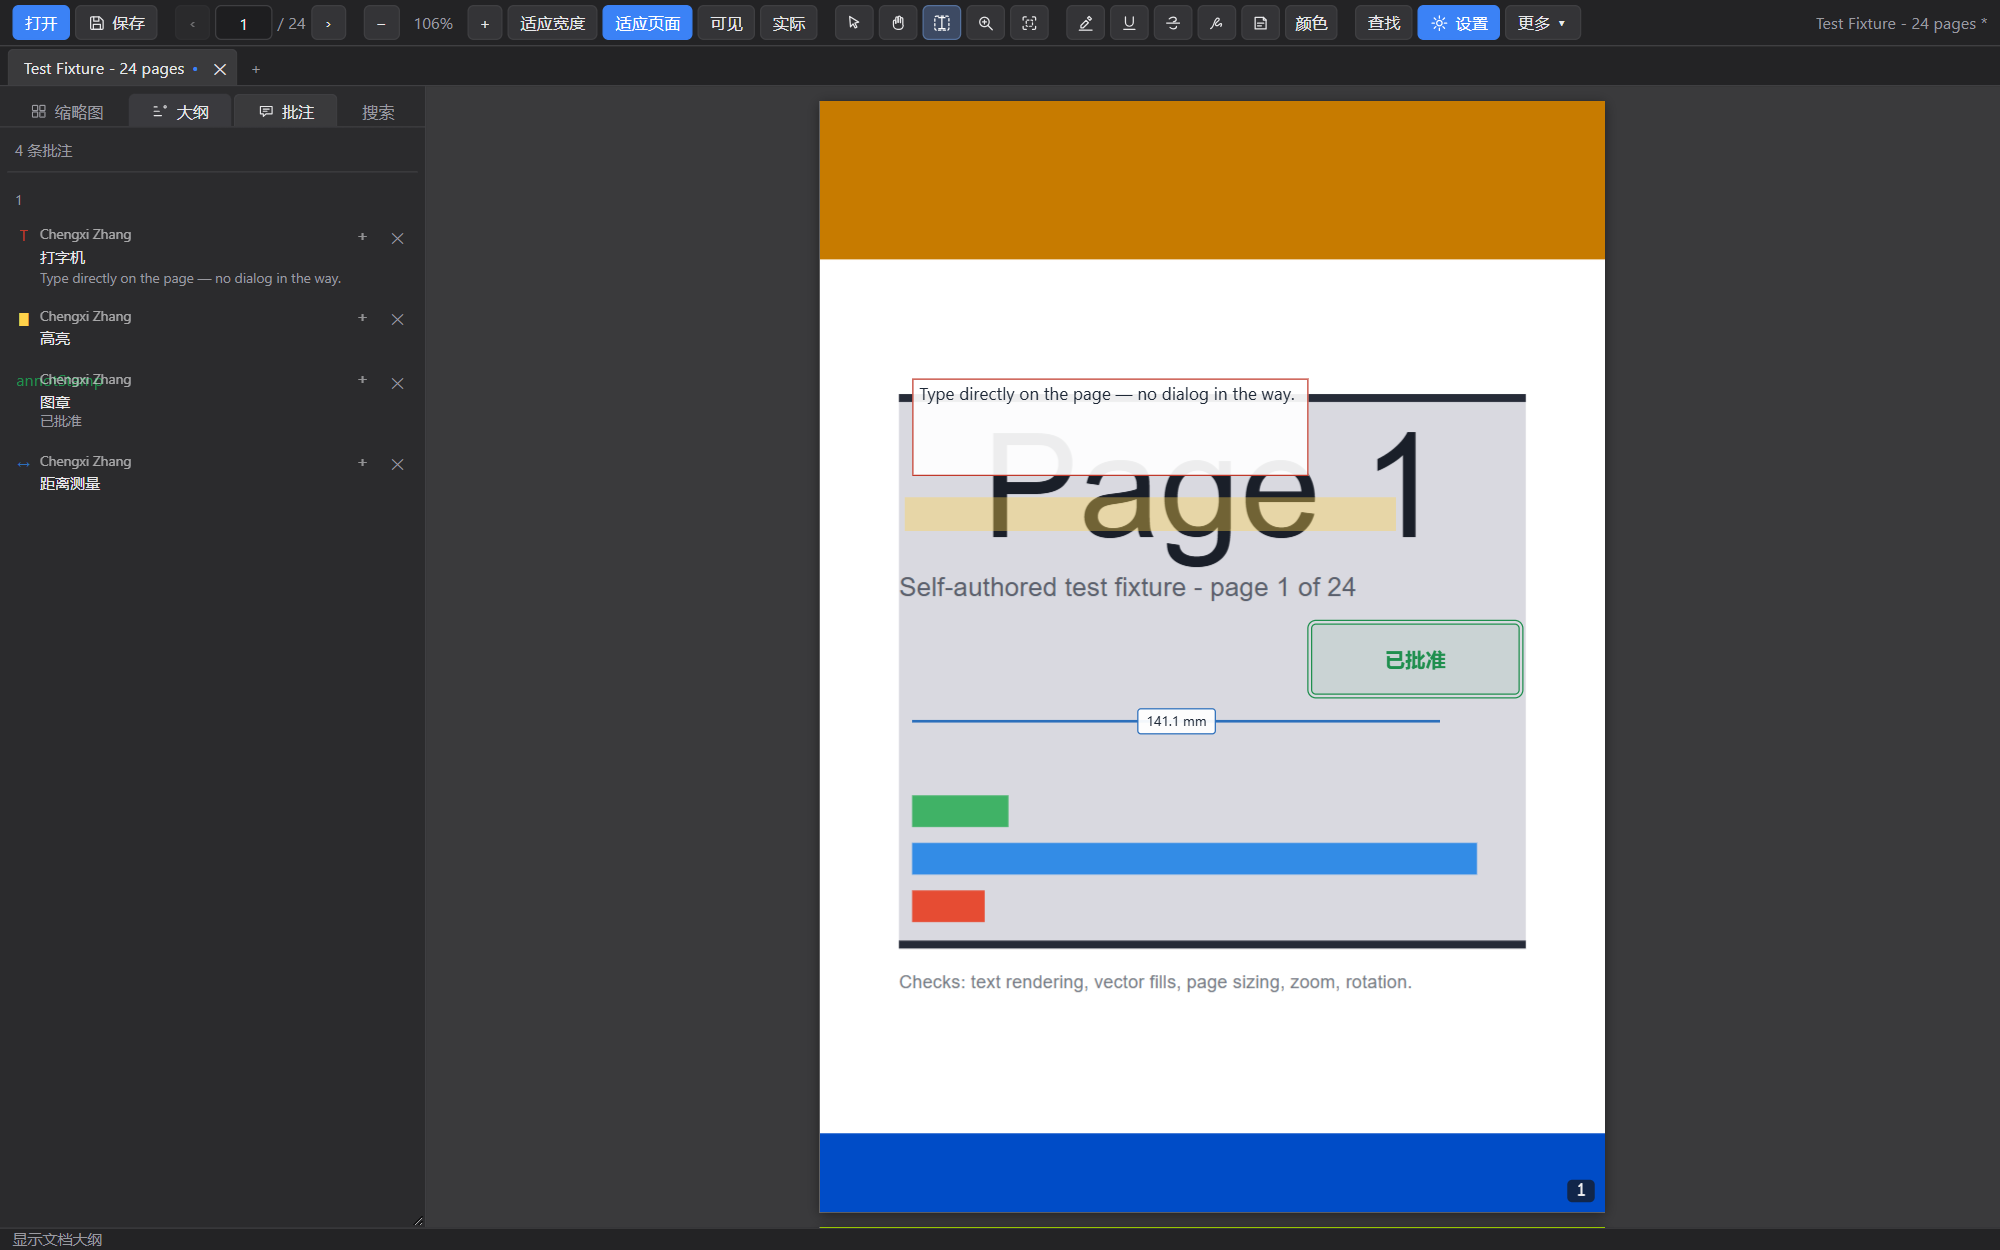
\includegraphics[width=\textwidth]{figures/screenshot.png}
  \caption{The application. The page carries a typewriter box, a text highlight, a standard
  stamp and a distance measurement; the sidebar lists them by kind, page and author. The
  panel matters as much as the page: an annotation that cannot be found again is not much of
  an annotation.}
  \label{fig:screenshot}
\end{figure}

\begin{table}[t]
  \centering
  \caption{Source size. Lines are physical lines of \texttt{.ts}, \texttt{.mjs},
  \texttt{.cjs} and \texttt{.css}; blank lines and comments are included, so the figures
  overstate logical code by roughly a fifth. Measured over the 47 application files and the
  52 test and tooling files.}
  \label{tab:modules}
  \small
  \begin{tabular}{@{}lrr@{}}
    \toprule
    Component & Files & Lines \\
    \midrule
    PDF reader and writers (\texttt{src/pdf}) & 8 & 3{,}349 \\
    Annotations (\texttt{src/annotations}) & 5 & 2{,}146 \\
    Viewer (\texttt{src/viewer}) & 5 & 1{,}334 \\
    UI, dialogs (\texttt{src/ui}) & 5 & 1{,}232 \\
    Tools: find, measure, snapshot (\texttt{src/tools}) & 5 & 972 \\
    i18n and command table (\texttt{src/i18n}) & 7 & 1{,}382 \\
    Sidebar panels (\texttt{src/sidebar}) & 4 & 738 \\
    Tabs and sessions (\texttt{src/tabs}) & 2 & 178 \\
    Saved searches (\texttt{src/search}) & 1 & 91 \\
    Styles & 1 & 1{,}414 \\
    Bootstrap (\texttt{main.ts}, \texttt{product.ts}) & 2 & 3{,}887 \\
    Electron host (\texttt{main.cjs}, \texttt{preload.cjs}) & 2 & 600 \\
    \midrule
    \textbf{Application} & \textbf{47} & \textbf{17{,}323} \\
    Tests and tooling (\texttt{tools/}) & 52 & 10{,}594 \\
    \bottomrule
  \end{tabular}
\end{table}

The 1{,}414 lines of CSS deserve a note: the application has four themes (light, dark, sepia,
high contrast) driven by custom properties on a \texttt{data-theme} attribute, which is why
the stylesheet is larger than several TypeScript modules. The 3{,}887-line bootstrap is the
concentration of failure in this architecture --- 91 commands, their bindings, the menu
descriptor, the debug hooks and the wiring of every module. It is also the file most likely to
be touched by a change, and the one where an omission is silent: a command registered without a
control appears in no menu and reports nothing.

\section{The PDF layer}
\label{sec:pdf-layer}

Five operations touch bytes: parse, incremental write (annotations), whole-document rewrite
(page operations), merge, and flatten (annotations baked into page content). They share a
parser and differ in what they are allowed to assume.

\subsection{Parsing}

The parser (\texttt{src/pdf/syntax.ts}, \texttt{document.ts}) handles the parts of ISO 32000
that real documents use: classic cross-reference tables, cross-reference streams, object
streams, incremental update chains via \texttt{/Prev}, and the standard filters for the
streams it must decode (none are decoded for a verbatim copy). It retains for every object
both the parsed value and, when the object was stored uncompressed, the exact source text.

The parsed value distinguishes streams by carrying their raw bytes:
\begin{lstlisting}[language={}]
type PdfStreamValue = {
  kind: 'stream';
  dict: PdfDict;
  raw: Uint8Array;   // exactly as it appears in the file, before any filter
};
\end{lstlisting}
This one field is what makes merging possible without a codec: a stream from another document
can be written back with its bytes untouched, because the only thing that needed rewriting
was the dictionary's references. See \S\ref{sec:merge}.

Two parser details caused defects worth recording, because both are invisible until a file is
written and re-read. First, an end-of-stream marker has two positions --- where the
\texttt{endstream} keyword begins and where its preceding newline ends --- and slicing content
with the trimmed one left a trailing newline that looked like the start of the next token.
Second, object numbers are not necessarily contiguous: a file may reference an object it does
not define, and the parser must distinguish ``missing'' from ``null'', since a page's
\texttt{/Annots} may legitimately be absent.

\subsection{The incremental annotation writer}
\label{sec:incremental}

Saving annotations appends objects to the existing file, rewrites the page dictionaries that
gained or lost annotations, and appends a cross-reference section whose trailer carries
\texttt{/Prev} pointing at the previous one. The original bytes are never modified, so the
operation is reversible by truncation and a reader that ignores the new section still sees a
valid document.

The invariant that governs everything is how a page's annotation array is computed. Let
$E$ be the object numbers currently listed in the page's \texttt{/Annots}, $R$ the object
numbers this writer produced for that page on the previous save, and $N$ the object numbers
of the annotations now in the model. Then

\begin{lstlisting}[language={}]
annots = [ refs(E) \ refs(R) ] ++ [ refs(N) ]
\end{lstlisting}

\noindent
and the page dictionary is rewritten whenever $N \cup R \neq \emptyset$ --- including when
$N = \emptyset$, because a page whose annotations were all deleted has no other reason to be
rewritten, and its \texttt{/Annots} would otherwise keep pointing at them.

\paragraph{What goes wrong without it.} The first implementation appended:
$\texttt{annots} = E \cup N$. Two symptoms followed, both reported by a user before any test
noticed.

\begin{enumerate}
  \item \textbf{Duplication.} Every save appended a fresh copy of every annotation on the page
        and listed both. Because the copies are byte-identical and coincide geometrically,
        the page looks correct; the file grows, and the reader may select one copy while
        deleting another. This reads to a user as ``the delete button does nothing''.
  \item \textbf{Resurrection.} A deleted annotation was removed from the model but its object
        was still listed in $E$, so the next save re-published it. The mark could not be
        removed from the document by any sequence of operations in the application.
\end{enumerate}

The fix records, per page, the object numbers the writer produced, keeps that map on the
document session, and passes it back on the next save as $R$; the writer uses the numbers it
produced this time as the new $R$. Objects superseded by earlier saves remain in the file as
orphans --- unreferenced, legal, and the price of never rewriting the original bytes.
\S\ref{sec:verification} describes the regression test, and a note on the test itself: the
first version of that test counted annotations in the file by calling the writer, which is a
write, so the counting added copies. It now fetches the saved file and resolves the page's
\texttt{/Annots}, counting what the file points at rather than what it contains.

\paragraph{Interoperability versus fidelity.} Every annotation is written twice, in a sense:
once as a standard annotation object that other readers display, and once as a private
\texttt{/PLP} dictionary holding this application's exact kind, stroke width, dash pattern and
font size. Standard subtypes cannot express all of it --- a text box and a callout are both
\texttt{/FreeText}, a replaced word is a \texttt{/StrikeOut} --- so the private entry is what
makes a round trip lossless. Section~\ref{sec:annot-model} discusses the cost of this duality.

\subsection{Whole-document rewrite}
\label{sec:rewrite}

Delete, insert, reorder, extract, crop and rotate pages cannot be expressed as an appending
update if they move pages between documents or change the page order: the page tree has to be
rebuilt. \texttt{rewritePdf} takes a plan --- for each output page, a source page index plus
optional rotation, crop box and a flatten step --- and produces a new file.

The invariant here is about \emph{inheritance}. In the source, a page may take
\texttt{MediaBox}, \texttt{CropBox}, \texttt{Resources}, \texttt{Rotate} and
\texttt{UserUnit} from an intermediate \texttt{/Pages} node. The rewrite produces a flat page
tree with one \texttt{/Pages} node, so each page must carry everything it inherited.
Omitting this does not fail: the file parses, and the pages are the wrong size, or sideways,
which is a far worse failure mode than an error.

Object handling follows from what the parser retained:

\begin{itemize}
  \item an object stored uncompressed is copied as its exact source text, with no
        re-serialisation, so anything the application does not model survives;
  \item an object inside an object stream is re-serialised from its parsed value, because its
        original bytes are inside a compressed container;
  \item a source page object is reused, and its dictionary rewritten, when that page appears
        exactly once in the plan; otherwise a fresh object is written;
  \item pages removed by the plan leave their objects unreferenced --- again legal orphans.
\end{itemize}

Because the plan can reference the same source page more than once, a rotation of a single
page is a one-page plan and a reorder is an identity plan with a permuted index list; the same
code path serves all of them.

\subsection{Merging two documents}
\label{sec:merge}

Merging is the one operation that copies between two object graphs. Every reference inside the
incoming document must be renumbered to its new home, or it will point at whatever the host
happens to keep at that number.

The algorithm is: build a map from each incoming object number to a fresh number above the
host's highest; for every incoming object except the page objects, its \texttt{/Pages} node
and its catalogue, re-serialise the value through a recursive reference rewrite, keeping
stream bytes and correcting \texttt{/Length} to the byte count; then build the incoming pages
on the host's page tree, with the same materialisation as \S\ref{sec:rewrite}.

Three details are easy to get wrong and were:

\begin{enumerate}
  \item \textbf{Stream bytes are not references.} A stream's data may contain any bytes,
        including ones that look like \texttt{N 0 R}. Only the dictionary is rewritten.
  \item \textbf{The incoming page tree is discarded, not merged.} Keeping the incoming
        \texttt{/Pages} node would leave a second tree with no parent, and readers differ on
        what to do with it.
  \item \textbf{Insertion is at a position, not an append.} Merging a cover sheet is the
        common case, so the interface takes a page index and clamps it to the document rather
        than rejecting it.
\end{enumerate}

\subsection{Flattening and summary documents}

\emph{Flattening} bakes annotations into page content: an extra content stream is appended
rather than merged into the existing one (a stream's bytes are immutable, and concatenating
inside one is a rewrite of bytes the writer promised not to touch), the page's
\texttt{/Annots} is dropped, and a Helvetica font is installed into a \emph{copy} of the
page's resource dictionary so the page's own font numbering is not disturbed.

\emph{Summarising} produces a new document containing the annotated pages. The obvious
implementation is a text listing of the comments, and it fails on the first document whose
comments are not in a Latin script: a text summary needs a font that covers whatever the
reader typed, and embedding one is a large amount of machinery for a summary. The
implementation instead renders each annotated page --- with its annotations already flattened
in --- at twice the page size and assembles the images into a new PDF. The result carries the
marks and the words inside them in any language, needs no font of its own, and costs nothing
that the printing path did not already provide.

\section{The annotation model}
\label{sec:annotations}

\subsection{Geometry}

An annotation stores its geometry in unrotated page space at scale~1, origin top-left, $y$
increasing downwards. Four consequences follow, all of them the reason for the choice:

\begin{itemize}
  \item a zoom changes a scale factor and nothing else;
  \item a rotation changes the transform used to paint, not the coordinates stored;
  \item a view-mode change (single, continuous, facing, facing-continuous) does not touch the
        model at all;
  \item hit testing compares a point in the same space, so it is a rectangle test rather than
        an inverse projection.
\end{itemize}

PDF user space is the mirror image, with an origin at the bottom-left and a scale given by the
page's \texttt{/UserUnit}, so writing an annotation is an explicit
\texttt{toScreen}/\texttt{fromScreen} conversion in one place
(\texttt{src/annotations/layer.ts}). Keeping that conversion in one function, rather than
inline at each use, is what made it possible to add rotated pages without auditing a dozen
call sites.

\subsection{Kinds and the dual representation}
\label{sec:annot-model}

Fifteen kinds are modelled. Twelve of them draw or carry text: highlight, underline,
strikeout, \emph{replace text}, freehand ink, sticky note, rectangle, ellipse, arrow,
typewriter (the original product's name for a free text box), callout text, and stamp --- where
stamp takes one of six standard names. The remaining three are measurements: distance,
perimeter and area.

Each is written as a standard subtype, so that other readers display it:
\texttt{/Highlight}, \texttt{/Underline}, \texttt{/StrikeOut}, \texttt{/Ink}, \texttt{/Text},
\texttt{/Square}, \texttt{/Circle}, \texttt{/Line}, \texttt{/FreeText}, \texttt{/PolyLine},
\texttt{/Polygon}, \texttt{/Stamp}. Alongside, a private \texttt{/PLP} dictionary carries
\texttt{/K} (the exact kind), \texttt{/W} (stroke width), \texttt{/D} (dash) and
\texttt{/F} (font size). Readers that do not know \texttt{/PLP} ignore it; this one prefers it
on load and falls back to inferring a kind from the subtype, which is how annotations made in
other applications are displayed with sensible defaults.

\paragraph{The cost of two representations.} This duality is the model's weakest point and
worth stating plainly. A third-party \texttt{/StrikeOut} with no \texttt{/PLP} becomes a
strikeout in this reader, which is correct; a \texttt{/StrikeOut} written by this reader for a
\emph{replace text} annotation becomes a strikethrough everywhere else, which is the closest
the format can express and is what the paper's \S\ref{sec:pdf-layer} describes as a
limitation rather than a feature. Two representations can also disagree --- a file edited in
another application may carry a \texttt{/PLP} kind that its subtype no longer supports --- and
the loader resolves that in favour of the subtype when the two are incompatible, silently. We
know of no such file; the rule exists because guessing in the other direction would be worse.

\paragraph{Threads.} A reply is its own annotation, a \texttt{/Text} object whose \texttt{/IRT}
points at its parent through an indirect reference; this is the mechanism every reader uses
to display a conversation. Reading back therefore takes two passes: a reply may reference a
parent that appears later in the page's list, so the loader collects replies first and attaches
them once every annotation is known. A reply whose parent lives on another page is still
shown, rather than dropped, because a missing parent is a fact about the file rather than
about the reply.

\paragraph{Identity and deletion.} Annotations carry a locally generated identifier and,
separately, the object number they were read from. The two must not be conflated: the
identifier survives an edit, while the object number is what a save must remove. Keeping the
second only on the document session, not on the annotation, is the design that made
\S\ref{sec:incremental} correct.

\subsection{Interaction}

Gestures are owned by the annotation layer rather than by the tool manager, because they
differ per kind: text markup consumes a selection, ink and rectangles drag out geometry, a
note is a single click, and a stamp is a click with a size of its own.

Two interaction rules were learned from defects:

\begin{itemize}
  \item \textbf{A click selects an annotation under any tool}, and the \emph{gesture} belongs
        to the active tool. An earlier version stopped propagation whenever a pointer landed on
        an annotation, which broke drag-to-scroll and marquee selection for gestures that
        merely started on top of a mark.
  \item \textbf{A text tool pressed on an existing text box edits it} rather than stacking a
        blank box on top. The earlier behaviour selected the annotation and then covered it with
        an empty box, which a user reasonably reported as ``I cannot select my annotation''.
\end{itemize}

\subsection{Rendering and printing}

Pages are virtualised: only pages near the viewport have a rasterised canvas, and a page
leaving the window drops its canvas while keeping its element. \S\ref{sec:eval} shows the
consequence in the measurements --- opening a 200-page document and a 24-page document take
the same time to first painted page.

Printing rasterises the selected range at twice the page size (144\,DPI) into a hidden
container, hides the application shell with a print stylesheet, and calls the platform's print
dialog; in the desktop build the same is done through the Electron main process. The printed
sheets are removed when the print job reports completion rather than on a timer, because a
timer loses the race on a slow printer.

\section{Search}
\label{sec:search}

\subsection{Matching and highlighting}

The document's text is not available as a string; it is a set of positioned glyph runs in a
text layer. The find index concatenates each page's run strings into one haystack and records
the run boundaries, so a match is an offset into a page's concatenated text plus a length.

Highlighting does not compute its own geometry. It rewrites the text layer's spans, splitting
a span at the match boundaries and wrapping the remainder in a \texttt{<mark>}-like element,
which is the technique pdf.js uses internally. The benefit is that a painted match is aligned
with the painted glyphs \emph{by construction}: there is no second coordinate computation that
could disagree with the first.

Because the index and the layer are separate, they can disagree. Before painting, the page's
live span strings are compared with the strings the index was built from; a page that does not
match is skipped rather than mis-highlighted. In practice this triggers when a page's text
layer is re-rendered between indexing and searching --- on a fast scroll through a document
whose index is still being built --- and skipping is the correct answer, since the offsets no
longer mean what they did.

\subsection{Result presentation}

Results are grouped by page, in document order, each row quoting the words around the match.
The quote comes from the index itself rather than from re-extracting the page: the offsets a
hit holds are offsets into exactly that string, so the snippet cannot drift from the
highlight.

Two ordering defects are worth recording because both produced a screen that contradicted
itself. First, the panel was told about a query \emph{before} the search ran, so it redrew from
the previous query's matches; because the zero-hit path returns early, nothing redrew
afterwards, and a search for nonsense left twenty-two results beside a status bar saying there
were none. Second, a match list is a view of mutable state: the ``current'' row must be
re-derived whenever the index changes, not only when the user moves to the next match.

\subsection{Folder search across documents}
\label{sec:folder-search}

Searching a folder means reading files the user has not opened. The application's desktop shell
refuses to read any path the user has not granted, so listing a folder also \emph{grants} the
files it finds: a folder the user types is as explicit a permission as one chosen from a
dialog, and the grant is what lets the scan proceed. Depth and file count are bounded, and a
file that will not parse is skipped rather than fatal --- one damaged document in a folder
should not stop the search.

Each file is opened on its own and released again. A folder search is a scan, not a shelf of
open documents; holding every parsed document would cost far more memory than it saves, and
\S\ref{sec:eval} shows the index is cheap enough to rebuild.

\subsection{Saved searches}

A saved search stores the question, not the answer: the query, the case and whole-word flags,
and the folder when there was one. The hits go stale the moment a document changes, and
re-running is the point. Saving under a name that already exists replaces it, so re-saving
updates rather than accumulating near-duplicates, and an entry with no name or no query is
dropped on read rather than repaired.

\subsection{Form fields, without a form layer}
\label{sec:fields}

The viewer highlights form fields --- tinting the rectangles of \texttt{/Widget} annotations so
a reader can see where a form asks for input --- and does not claim to fill them. The
distinction matters for the paper because it is the honest boundary of the feature: detecting
a widget needs the page's annotation array, while filling one needs the field's own hierarchy
(an \texttt{/AcroForm} dictionary, field types, appearance streams, calculation order and
validation), which this application does not implement. Highlighting without filling is
useful and truthful; a half-implemented form layer would be neither.

\section{Verification}
\label{sec:verification}

\subsection{What is asserted}

The project has no unit-test pyramid. It has \textbf{31 suites of behavioural assertions},
each of which drives the real application --- a real browser for the renderer, the real
packaged executable for the desktop build --- and then asks questions of what it produced:
pixels, bytes, and document model state.

The choice follows from where the defects were. In a system that parses, rewrites and
re-parses a binary format, the interesting failure is rarely a wrong return value; it is a file
that opens and is wrong. Two examples from the suites:

\begin{itemize}
  \item After a save and a reopen, a text annotation is clicked with a real mouse and the
        assertion is that the annotation is selected and shows a resize grip --- not that a
        function returned an object.
  \item After flattening, the styled text is sampled from the rendered canvas at the
        coordinates the annotation occupied, and the sampled colour must be the annotation's
        colour. A flattening bug that wrote the operators in the wrong coordinate system
        produces a valid file and fails this assertion.
\end{itemize}

Snapshots are deliberately not used: they would freeze rendering differences between browser
versions and say nothing about whether a saved file is correct.

\subsection{Two targets}

The renderer is verified in a headless browser; the desktop shell is verified by launching the
packaged executable through Playwright's Electron support. Both are necessary because they fail
differently. The browser build exercises the code paths a web deployment would take, and the
packaged build is the only place where file dialogues, native menus, window geometry memory and
the print path through the main process exist at all.

The split, measured, is 734 assertions over 28 suites for the browser build and 55 over 3
suites for the packaged application; Table~\ref{tab:suites} groups them.

\begin{table}[t]
  \centering
  \caption{The verification suites, grouped. The per-suite breakdown is in the repository
  (\texttt{paper/\allowbreak metrics/\allowbreak results.json}, produced by \texttt{tools/\allowbreak collect-metrics.mjs}).}
  \label{tab:suites}
  \small
  \begin{tabular}{@{}lrr@{}}
    \toprule
    Group & Suites & Assertions \\
    \midrule
    Foundations: resource container, embedded font, i18n packs & 3 & 78 \\
    Reading and interface: layout, view modes, zoom, print, themes, tabs & 9 & 297 \\
    PDF writing: incremental save, round trip, rewrite, page operations, merge & 8 & 202 \\
    Annotations: author, stamp, reply, replace, flatten, summary, fields & 6 & 116 \\
    Search: in-document, saved & 2 & 41 \\
    \midrule
    Browser build & 28 & 734 \\
    Packaged application & 3 & 55 \\
    \midrule
    \textbf{Total} & \textbf{31} & \textbf{789} \\
    \bottomrule
  \end{tabular}
\end{table}

\subsection{Defects the methodology caught}

\paragraph{The one it did not catch first.} The annotation duplication and resurrection
described in \S\ref{sec:incremental} was reported by a user after release, not found by the
suites. The reason is instructive: the round-trip suite asserted that annotations survived a
save and reopen --- which they did, twice over. Nothing asserted that saving \emph{twice}
changed nothing, and nothing asserted that a deleted annotation was gone from the file. Both
assertions now exist, in \texttt{e2e-save-reopen}: save two, reopen, click one, save twice
more, delete one, save, reopen, delete the last, save, reopen.

\paragraph{Defects in the harness itself.} Three failures were in the measurement rather than
the product, and all three are worth recording because each produced a confident wrong answer.

\begin{enumerate}
  \item \textbf{Counting by writing.} The first version of the regression test counted the
        annotations in the saved file by calling the writer. The writer appends, so the act of
        counting added a copy, and the test failed for a reason of its own making. The test now
        fetches the saved bytes and resolves the page's \texttt{/Annots}, which counts what the
        file \emph{points at} rather than what it contains.
  \item \textbf{Testing the projection.} Two features --- an annotation author and a stamp name
        --- were briefly diagnosed as broken because the test read state through a hand-written
        debug projection that listed a fixed set of fields, and the projection had not been
        extended. The feature worked; the projection lied. This is the most expensive mistake
        in the project's history, because it is invisible: a projection tested through itself
        proves only that the projection works. The rule now is that assertions read the
        document model directly wherever a hook is not the thing under test.
  \item \textbf{An unwritten fixture.} Continuous integration went red for three consecutive
        commits because the fixtures a suite opens are generated by a script, the fixture
        directory is intentionally not committed, and a new generator had not been added to
        that script. The suite timed out waiting for a page that was never served. The CI log
        named the suite; nothing named the cause.
\end{enumerate}

\paragraph{The limits of the harness.} Two are known and reported rather than papered over.
Synthetic mouse-button events do not reach the packaged window through the automation layer, so
the packaged suite asserts what the harness can prove (the tool is selectable, the region
exists) and does not claim to have dragged anything. And the window-geometry assertion is
stateful: it fails when three suites run back to back with the process killed between them and
passes when run alone, because it reads geometry a previous run wrote.

\subsection{Reproducing the numbers}

Every figure in this paper comes from a script in the repository, not from a notebook.
\texttt{tools/\allowbreak collect-metrics.mjs} runs the 31 suites and parses each one's summary line into
\texttt{paper/\allowbreak metrics/\allowbreak results.json}; \texttt{tools/\allowbreak benchmark.mjs} produces the timings in
Table~\ref{tab:timings} and writes \texttt{paper/\allowbreak metrics/\allowbreak benchmark.json}. Both refuse to guess:
a suite that fails is recorded as failing and a timing that cannot be taken is \texttt{null}.

\section{Evaluation}
\label{sec:eval}

\subsection{What is measured, and what is not}

Three things are measured: the size of the system, the size of what ships, and the wall-clock
cost of the operations the paper describes. All three are taken from the artefact on one
machine (Windows 11, Node 24, an x86-64 desktop CPU) with the scripts named in
\S\ref{sec:verification}.

We do \textbf{not} report a comparison against other readers, and the reason is not modesty.
A fair comparison would need a matched document corpus, a defined set of tasks, and a
measurement of correctness as well as speed --- and this system has no claim to be faster than
an engine written in C. What the numbers below establish is narrower and, we think, more
useful: that the writing operations are cheap enough to run on every save, and that
virtualisation makes open time independent of document length.

\subsection{Size}

\begin{table}[t]
  \centering
  \caption{What ships. The unpacked executable is the application plus the Electron runtime;
  the renderer bundle is the code this paper describes.}
  \label{tab:sizes}
  \small
  \begin{tabular}{@{}lr@{}}
    \toprule
    Artefact & Size \\
    \midrule
    Renderer bundle, JavaScript & 660.2\,kB (197.8\,kB gzip) \\
    Renderer bundle, CSS & 26.1\,kB (6.0\,kB gzip) \\
    UI resource container & 19.0\,kB \\
    Application source & 17{,}323 lines over 47 files \\
    Test and tooling source & 10{,}594 lines over 52 files \\
    \midrule
    Portable executable (single file) & 108.1\,MB \\
    Unpacked executable & 235.6\,MB \\
    \bottomrule
  \end{tabular}
\end{table}

Table~\ref{tab:sizes} separates two facts that are usually conflated. The code this paper
describes is 198\,kB compressed; the download is 108\,MB, and 99.8\,\% of it is the Electron
runtime. That ratio is a property of the packaging choice, not of the application, and it is
the project's largest engineering compromise: a native shell would ship a few megabytes and
cost months of platform work.

The test-to-application line ratio is 0.61:1. We report it because it is a design choice with
a cost --- a tenth of the codebase exists to check the other nine tenths --- and because a
figure that low is only defensible if the suites assert behaviour rather than implementation,
which \S\ref{sec:verification} argues they do.

\subsection{Cost of the writing operations}

\begin{table}[t]
  \centering
  \caption{Measured cost of the operations this paper describes, in the renderer, excluding
  file I/O. Median of repeated runs on fixtures of 24 and 200 pages; the raw samples are in
  \texttt{paper/\allowbreak metrics/\allowbreak benchmark.json}.}
  \label{tab:timings}
  \small
  \begin{tabular}{@{}lrr@{}}
    \toprule
    Operation & Document & Median \\
    \midrule
    Open to first painted page & 24 pages & 271\,ms \\
    Open to first painted page & 200 pages & 279\,ms \\
    Build full-text index & 24 pages & 4.9\,ms \\
    Build full-text index & 200 pages & 40.9\,ms \\
    Incremental annotation save & 24 pages & 1\,ms \\
    Whole-document rewrite & 24 pages & 2\,ms \\
    Merge two 24-page documents & 48 pages out & 3\,ms \\
    JavaScript heap after opening & 200 pages & 7\,MiB used \\
    \bottomrule
  \end{tabular}
\end{table}

Two rows carry the paper's practical argument.

\paragraph{Open time is independent of length.} 271\,ms for 24 pages and 279\,ms for 200 pages
--- a 3\,\% difference across an eight-fold increase in document size. This is what
virtualisation is for: the application rasterises the pages near the viewport and nothing else,
so the cost of opening is the cost of the first screen plus parsing the cross-reference, not
the cost of the document.

\paragraph{Writing is cheap enough to do on every save.} An incremental save of a 24-page
document is around a millisecond; a full rewrite of the same document is two; merging two
24-page documents into 48 is three. These are single-digit milliseconds for operations that
earlier sections described as delicate, which is the useful observation about the design: the
difficulty was never performance, and the invariants in \S\ref{sec:pdf-layer} cost nothing to
uphold. A save can therefore be conservative --- rewrite the page's annotation array, drop the
objects it replaces, write a fresh cross-reference --- rather than clever.

The index figure scales linearly: 4.9\,ms for 24 pages, 40.9\,ms for 200, i.e.\ about
0.2\,ms per page. That is why folder search rebuilds an index per file rather than storing one
(\S\ref{sec:folder-search}), and why the 7\,MiB heap figure for a 200-page document is
consistent with holding no more than the pages near the viewport.

\subsection{Threats to validity}

The measurements are from one machine and one rendering engine, and the electron and browser
versions are pinned only by \texttt{package.json} ranges. The timings are in-process and exclude
disk and IPC, so they understate what a user waits for on a save; the open-time figures include
navigation and first paint, so they overstate what a second open of the same file costs.

The assertion count is a measure of effort, not of coverage. There is no instrumentation-based
coverage figure in this paper because none was collected; a suite count can be raised by
writing easier tests, and the reader should treat 789 as evidence that many behaviours are
checked, not as a percentage of the behaviours that exist.

\section{Discussion, limitations and conclusion}
\label{sec:discussion}

\subsection{What generalises}

Three lessons seem portable beyond this application.

\paragraph{An incremental format turns every writer into a stateful operation.} The bug in
\S\ref{sec:incremental} is not a coding error in the ordinary sense; it is a failure to model
the writer as having a \emph{past}. A function that appends is correct once, so any provider of
such a function must answer the question ``what did you write last time?'' The answer in this
system is a per-page set of object numbers held on the document session, and the general
statement is that the state belongs next to the bytes, not inside the writer.

\paragraph{Flattening a tree materialises inheritance.} This is true of any format with
inheritable attributes --- CSS, DOM, scene graphs, PDF page trees. The failure is silent
because the flattened document is still well-formed; the flaw is that it means something else.

\paragraph{A test can be wrong in a way that looks like a finding.} The projection trap in
\S\ref{sec:verification} cost the project more time than any product defect, twice, on the same
feature pattern. The rule we now apply --- assert against the model, not against a debug
surface that describes the model --- is cheap and should have been adopted on the first
occurrence.

\subsection{Limitations}
\label{sec:limits}

This list is the boundary of what the paper's claims cover.

\begin{itemize}
  \item \textbf{No installer and no code signing.} The application ships as a portable
        executable; Windows SmartScreen warns on first run. Fixing this needs a code-signing
        certificate, not code.
  \item \textbf{Windows only.} The packaged target is Windows x64. Nothing in the renderer is
        platform-specific, but the shell is not exercised elsewhere.
  \item \textbf{Encrypted documents are refused for writing.} They open for reading through the
        renderer; an annotation save against an encrypted file is rejected rather than
        attempted.
  \item \textbf{Files grow with every save.} The incremental writer never rewrites the original
        bytes, so superseded objects remain as orphans. A compaction pass would need a
        whole-document rewrite and is not implemented.
  \item \textbf{Flattening cannot encode text outside Latin-1.} The embedded appearance font is
        a standard Helvetica; a flatten of Chinese or Greek annotation text renders as
        placeholders. The summary feature avoids this by rendering pages instead of writing
        text (\S\ref{sec:pdf-layer}).
  \item \textbf{No form filling, digital signatures or OCR.} Form fields are highlighted, and
        \S\ref{sec:fields} is explicit about why that is not the same as supporting forms.
  \item \textbf{Replace text is written as \texttt{/StrikeOut}}. The format has no replace-text
        annotation type; another reader shows the strike and not the substitution, which is
        visible in the PDF and correct, and incomplete as a representation of the intent.
  \item \textbf{One machine, one engine.} The timings come from a single Windows host and a
        single pdf.js version.
  \item \textbf{Rendering quality is not evaluated.} The application delegates rasterisation to
        pdf.js; any rendering difference the reader observes is the engine's, not this
        project's, and the paper makes no claim either way.
\end{itemize}

\subsection{Conclusion}

A PDF reader that writes is a different system from a PDF reader that renders, and the
difference is concentrated in a small number of invariants that are easy to state and easy to
break: rebuild a page's annotation array rather than appending to it; materialise what a page
inherits before flattening its tree; renumber references when copying between documents and
leave stream bytes alone. Each invariant, violated, produces a file that opens and is wrong ---
which is why the verification described here asks questions of pixels and bytes rather than of
return values, and why the paper reports the defects that reached a user as well as the ones
the suites caught.

The application is 17{,}323 lines of source over 47 files with one runtime dependency, MIT
licensed, and available with its tests and the scripts that rebuilt every figure here at \repo.

\section*{Acknowledgements}

The software described here was developed with the assistance of \textbf{DeepSeek AI} and of
\textbf{DSH} (DeepSeek Harness), the agent harness built on it, and this preprint was
researched, drafted and revised with the same assistance. The debt is not incidental to the
result. The invariant that makes annotation deletion work (\S\ref{sec:incremental}), the
decision to materialise inheritance before flattening a page tree (\S\ref{sec:rewrite}), and
the harness defects recorded in \S\ref{sec:verification} were all arrived at in the course of
that collaboration, and the manuscript was argued out the same way.

It is in that spirit --- and because a program that expects its behaviour to be checked should
let its readers check it --- that all of this software is released as open source, with nothing
held back. The disclosure is deliberate: a reader is entitled to know how a document was
produced, as a reader of the source is entitled to see every line of it.

The dual representation of \S\ref{sec:annotations}, the coordinate convention and the decision
to write into the document rather than beside it came from using the software daily while
building it. The pdf.js project~\cite{pdfjs} does the rendering; the writer's invariants were
learned by breaking them.

I thank Liang Shengren, and this remarkable era, in which such an undertaking is within
reach of one person with a laptop and a good interlocutor.



% An inline bibliography rather than BibTeX: one fewer tool in the build, and arXiv's
% compiler runs the same two passes the authors did.
% Inline bibliography: no BibTeX pass, so two pdflatex runs are the whole build.
\begin{thebibliography}{9}
\small
% References are set a size down with tight item spacing: it is conventional, and it
% keeps a nine-entry list from spilling a single line onto a page of its own.
\setlength{\itemsep}{1pt}

\bibitem{iso32000}
International Organization for Standardization.
\newblock {\em ISO 32000-1:2008 --- Document management --- Portable Document Format ---
  Part 1: PDF 1.7}, 2008.

\bibitem{pdfjs}
Mozilla.
\newblock {\em pdf.js: a PDF renderer for the web}.
\newblock Apache License 2.0. \url{https://mozilla.github.io/pdf.js/}

\bibitem{mupdf}
Artifex Software.
\newblock {\em MuPDF: a lightweight PDF, XPS and eBook rendering library}.
\newblock Dual licensed AGPL v3 / commercial. \url{https://mupdf.com/}

\bibitem{okular}
The KDE Community.
\newblock {\em Okular: the KDE universal document viewer}.
\newblock \url{https://okular.kde.org/}

\bibitem{pdfbox}
The Apache Software Foundation.
\newblock {\em Apache PDFBox: a Java library for working with PDF documents}.
\newblock Apache License 2.0. \url{https://pdfbox.apache.org/}

\bibitem{pdfxchange}
Tracker Software Products.
\newblock {\em PDF-XChange Viewer}.
\newblock Commercial Windows application, development discontinued.
\newblock \url{https://www.tracker-software.com/}

\bibitem{electron}
OpenJS Foundation.
\newblock {\em Electron: build cross-platform desktop applications with JavaScript, HTML and
  CSS}.
\newblock MIT License. \url{https://www.electronjs.org/}

\bibitem{vite}
Evan You and contributors.
\newblock {\em Vite: a frontend build tool}.
\newblock MIT License. \url{https://vite.dev/}

\bibitem{playwright}
Microsoft.
\newblock {\em Playwright: browser and Electron automation}.
\newblock Apache License 2.0. \url{https://playwright.dev/}

\end{thebibliography}


\end{document}
